%%%% SEITENRAENDER, SCHRIFTGROESSE UND ZEILENABSTAND NICHT ABAENDERN => SONST GIBT ES PUNKTEABZUG
\documentclass[a4paper,11pt,singlespacing]{article}
\usepackage[left=2.5cm,right=2.5cm,top=2.5cm]{geometry}
\usepackage{setspace}
\usepackage[utf8]{inputenc}
\usepackage{graphicx}
\usepackage{color}
\usepackage{hyperref}
\usepackage{biblatex}

\usepackage{listings,xcolor}
%opening
\title{DockerSec: Cybersecurity Training and Testing Environment}
\author{
	Rémi JARDRET 20741372,
	Stéphane SIMON 21641381
	}


\begin{document}
% Absatzeinrückung verhindern
\setlength{\parindent}{0ex}


\begin{titlepage}
	
	\newcommand{\HRule}{\rule{\linewidth}{0.5mm}} % Defines a new command for the horizontal lines, change thickness here
	
	\center % Center everything on the page
	
	%----------------------------------------------------------------------------------------
	%	HEADING SECTIONS
	%----------------------------------------------------------------------------------------
		
	
	
\includegraphics[width=7cm]{images/rwu_logo.png}\\[1.5cm] % Include a department/university logo - this will require the graphicx package
	
	\textsc{\LARGE University of Applied Sciences Ravensburg Weingarten}\\[1.5cm] 
	\textsc{\Large Department of
		Electrical Engineering
		and Computer Science}\\[0.5cm]
	\textsc{\large Bachelor Project}\\[0.5cm] 
	
	%----------------------------------------------------------------------------------------
	%	TITLE SECTION
	%----------------------------------------------------------------------------------------
	
	\HRule \\[0.4cm]
	{ \huge \bfseries DockerSec: Cybersecurity Training and Testing Environment}\\[0.4cm] 
	\HRule \\[3.5cm]
	
	%----------------------------------------------------------------------------------------
	%	AUTHOR SECTION
	%----------------------------------------------------------------------------------------
	
	\begin{minipage}{0.4\textwidth}
		\begin{flushleft} \large
			\emph{Author:}\\
   			Rémi \textsc{JARDRET}\\
			20741372\\
			Stéphane \textsc{SIMON}\\
			21641381
		\end{flushleft}
	\end{minipage}
	~
	\begin{minipage}{0.4\textwidth}
		\begin{flushright} \large
			\emph{Supervisor:} \\
			Herr Benjamin \textsc{Stähle}\\ % Supervisor's Name
            \& \\
			Herr Norbert \textsc{Perk} % Supervisor's Name
		\end{flushright}
	\end{minipage}\\[5cm]
	
	% If you don't want a supervisor, uncomment the two lines below and remove the section above
	%\Large \emph{Author:}\\
	%John \textsc{Smith}\\[3cm] % Your name
	
	%----------------------------------------------------------------------------------------
	%	DATE SECTION
	%----------------------------------------------------------------------------------------
	
	{\large \today}\\[5cm] % Date, change the \today to a set date if you want to be precise
	
	%----------------------------------------------------------------------------------------
	%	LOGO SECTION
	%----------------------------------------------------------------------------------------

	%----------------------------------------------------------------------------------------
	
	\vfill % Fill the rest of the page with whitespace
	
\end{titlepage}


\tableofcontents
\pagebreak

%%%% TITLES AND CONTENTS %%%%
\section{Context}
This project has its roots in our Linux Administration course at our home institution. In this course, we were tasked with creating an environment comprising a minimum of six virtual machines (VMs) running different Linux distributions. However, this turned out to be a labor-intensive process that required a significant amount of hardware resources.\par
On the other hand, we also attended classes in cybersecurity, specifically pentesting, where we frequently encountered similar environments. In these classes, we often found ourselves spending approximately three sessions setting up the environment before we could commence our training and pentesting.\par
Following this observation, we concluded that a pre-configured environment with optimized resource utilization would be highly beneficial. Ideally, this environment should be quick and easy to set up. Docker, and particularly Docker Compose, emerged as the perfect solution, offering a streamlined and state-of-the-art approach.\par
This project is part of an Erasmus exchange program and is taking place during the Linux Administration course at the RWU. The subject matter not only holds potential value for the RWU but also for future students. As part of the Erasmus experience, we aim to create a solution that not only streamlines our coursework but can be a valuable resource for students and beyond.\par



\section{Objectives}
This project is driven by several key objectives, each addressing specific challenges and needs:

\begin{enumerate}
    \item \textbf{Streamlined Environment Setup:} One primary objective is to eliminate the time-consuming and intricate setup of environments for learning and training purposes. The current process of configuring multiple virtual machines (VMs) running different Linux distributions can be arduous, and we aim to simplify this.
    
    \item \textbf{Ease of Deployment:} We also seek to address the challenges related to setting up these environments, making it more user-friendly. The configuration of complex network topologies, including DHCP, DNS, HTTP servers, DMZs, firewalls, and routers, can be daunting for learners and security enthusiasts.
    
    \item \textbf{Resource Optimization:} Resource optimization is a crucial goal. We want to ensure that the environment we provide is efficient in terms of resource utilization, enabling users to run multiple instances simultaneously without overwhelming hardware resources.
\end{enumerate}

Taking these overarching objectives into account, we have defined three specific goals for our project:

\begin{itemize}
    \item \textbf{Facilitating System Administration Learning:} We aim to create an environment where users can explore and understand the intricacies of system administration. This involves gaining insights into the setup and configuration of different components such as "computers," networks, and services. Users can investigate, extend, and experiment with various aspects of system administration.

    \item \textbf{Enhancing Pentesting Training:} Our project seeks to provide a robust platform for pentesting training. This environment will enable users to practice various types of attacks, such as spoofing, scanning, and brute-forcing... Almost all of the Cyber Kill Chain\footnote{https://www.lockheedmartin.com/en-us/capabilities/cyber/cyber-kill-chain.html} can be experimented on this environment.

    \item \textbf{Exploring Docker Capabilities:} This project will serve as an exemplary case among many, enabling learners to delve into more complex Docker setups and explore the full extent of Docker's capabilities.

\end{itemize}

In practical terms, our project aims to deliver an environment consisting of Linux-based machines with integrated features, that will we detail in the next part. This environment will serve as a multifaceted learning platform. Users can look at the configurations, experiment with various scenarios, and advance their knowledge in both system administration and cybersecurity. With the ability to simulate attacks, the project aims to offer an arena for learning and practice.

\section{Requirements}
As mentionned in our previous document called "Project Sketch", we will deploy the following infrastructure (Appendix \ref{Appendix1} )

\subsection{Functional Requirements}
From a functional perspective, this environment is designed to provide a scalable and efficient platform for cybersecurity training and Linux administration testing. The primary objective is to achieve a noticeable reduction in host system resource utilization when compared to traditional setups using virtual machines.\par

In addition to energy efficiency, this environment should be readily operational with a simple "docker compose" command, emphasizing ease of deployment. Rigorous testing is essential to identify and address potential system-specific issues, ensuring seamless functionality. The initial focus is on enabling deployment on Unix host systems, with a secondary objective to extend compatibility to Windows host systems.\par

Furthermore, this project aims to be a valuable learning resource. Both pentesters and Linux administrators should be able to acquire knowledge through this environment. This necessitates the inclusion of diverse scenarios, ranging from basic cybersecurity spoofing attacks to advanced system hacking and denial of service simulations. For Linux administrators, the environment must provide real-world scenarios, including DNS configuration, Apache setup, DHCP server management, and more.\par

\subsection{Technical requirements}
For the technical requirements of the DockerSec project, the following specifications and technologies will be used:
\begin{itemize}
    \item \textbf{Containerization with Docker:} The project will use Docker for containerization. Docker containers will be used to encapsulate various services, applications, and components to ensure consistency and portability across different host systems.

    \item \textbf{Macvlan Network Technology:}  Macvlan network technology will be employed to assign distinct IP and MAC addresses to each container for network isolation. This technology will enable the creation of a realistic network environment, including the implementation of a DMZ (Demilitarized Zone) and subnetworks. The use of Macvlan ensures that each container behaves like an individual machine with its own network identity, making it possible to establish DMZs and subnetworks for practicing more advanced network configurations and security scenarios.
    
    \item \textbf{Security and Isolation:} The DockerSec environment must ensure security and isolation between containers and network components to prevent unintended interactions and breaches. This is crucial for conducting realistic pentesting scenarios safely..
   
    \item \textbf{Attack Simulation with Eve:} The attacker, Eve, will be deployed both inside and outside the network for simulating various attack scenarios. This involves setting up containers to represent Eve, the attacker, to practice different types of attacks like spoofing, scanning, brute-forcing, and other pentesting activities.

    \item \textbf{Linux-Based Containers:} The project will use Linux-based containers to replicate the Linux operating system environment, including various distributions, services, and configurations commonly encountered in Linux administration and cybersecurity training.

    \item \textbf{Docker Compose for Orchestration:} Docker Compose will be used to define and orchestrate the composition of multiple Docker containers. It simplifies the deployment and management of complex multi-container applications, allowing users to define services, networks, and volumes in a single YAML file.

    \item \textbf{Realistic Network Topology:} The project will aim to create a realistic network topology that includes elements such as routers, firewalls, DNS servers, DHCP servers, and web servers. It is imperative that these network components are configured to ensure the functional operation of web services. This will help users explore and practice real-world scenarios in system administration and pentesting by interacting with services that are not only present but fully functional within the network environment.

 


\end{itemize}
These technical requirements will form the foundation of the DockerSec project, enabling the creation of a comprehensive cybersecurity training and testing environment using Docker containers and advanced network configurations.

\section{Project Management}
\subsection{Timeline}
As previously mentioned in our project context, the project is scheduled for the winter semester of 2023, which aligns with our Erasmus semester. Throughout the entire semester, we will employ an agile project management methodology, specifically Kanban. Using GitLab's features, such as to-do lists, feature requests, and task tracking, we will maintain real-time visibility into the project's progress, what has been accomplished, and what remains to be done.\par

This agile project management approach will enable us to set and achieve specific project milestones. These milestones will be visualized in the GANTT diagram, available in Appendix \ref{Appendix2}.\par

In addition to this planning, we plan to do some team meetings regularly and progress updates. Allowing us to adjust the timeline planned if we have any kind of delays or main issues.\par 

\subsection{Roles}
Our project team consists of Rémi JARDRET and Stéphane SIMON, each bringing their skill set to the project. Rémi's expertise lies in networking, bolstered by his CCNA certifications. Stéphane, on the other hand, possesses a lot of experience with Docker and Kubernetes environments. Both of us are pursuing studies in ethical hacking, and we will assume the following roles in this project:

\begin{enumerate}
    \item Rémi: Network setup and testing, development of pentesting scenarios.
    \item Stéphane: Design and deployment of the Docker environment, development of pentesting scenarios.
\end{enumerate}

\subsection{Resources}
To ensure the success of this project, we will have access to a dedicated repository on the university's GitLab platform. This repository will serve as a central hub for our project, facilitating various aspects of our agile project management, providing a backup of our work, and enabling us to monitor progress.\par
Furthermore, the university will provide us with access to designated rooms equipped with desktop computers. Additionally, our teachers will be available on Thursday afternoons to provide guidance and support whenever needed. We can also use the GitLab issue tracking system to promptly notify our teachers of any challenges or issues that may arise during the project.\par

\section{Constraints}
The DockerSec project operates within a specific set of constraints:\par
Time Constraints: The project is scheduled to run from October to December. This limited time frame presents a challenge in terms of project planning and execution. Ensuring that all project objectives are met within this relatively short period requires efficient time management and a focus on prioritizing key tasks.\par
Technical Constraints: It's important to note that Docker, which will be used for the project, is generally considered to be less secure than a traditional Virtual Machine (VM).
Docker containers share the same kernel with the host operating system, which can introduce potential security vulnerabilities. In a VM, on the other hand, there is a clear separation between the guest OS and the host OS, providing stronger isolation and security.\par
While DockerSec will implement security best practices and network isolation measures, it's essential to acknowledge this inherent difference in security models. Therefore, a risk assessment and appropriate security configurations must be a part of the project to minimize any potential security risks associated with Docker.\par
Furthermore, Docker is a community-driven solution that evolves constantly. Each tweak or workaround used to address a specific issue or to achieve a certain configuration may be better handled by future updates.\par
These constraints guide the project's planning and execution, necessitating a focus on efficient time management, resource optimization, and creative solutions that align with the educational context and available resources.\par

\section{Deliverables}
During the course of this project, we will deliver the following:

\begin{enumerate}
    \item The final report: a document to be written and submitted to the instructors in accordance with the established timetable and requirements of the teachers.
    
    \item Project behavior documentation: a comprehensive document describing the project's behavior to facilitate understanding, enabling the project to be extended or reused.
    
    \item Main scenarios documentation: documents outlining the main pentesting scenarios to aid in comprehension.
\end{enumerate}

In addition to these documents, we will provide the following:

\begin{enumerate}
    \item GitLab repository: containing all the project work.
    
    \item docker-compose.yml files: with the docker environment configuration.
    
    \item DOCKERFILE: to recreate container images locally.
    
    \item If necessary, a shell installation script.
\end{enumerate}


%%%% APPENDICES %%%%
\newpage
\section{Appendices}


\subsection{Appendix 1 : Project's Architecture}
\label{Appendix1}
\begin{figure}[bp!]
    \centering
    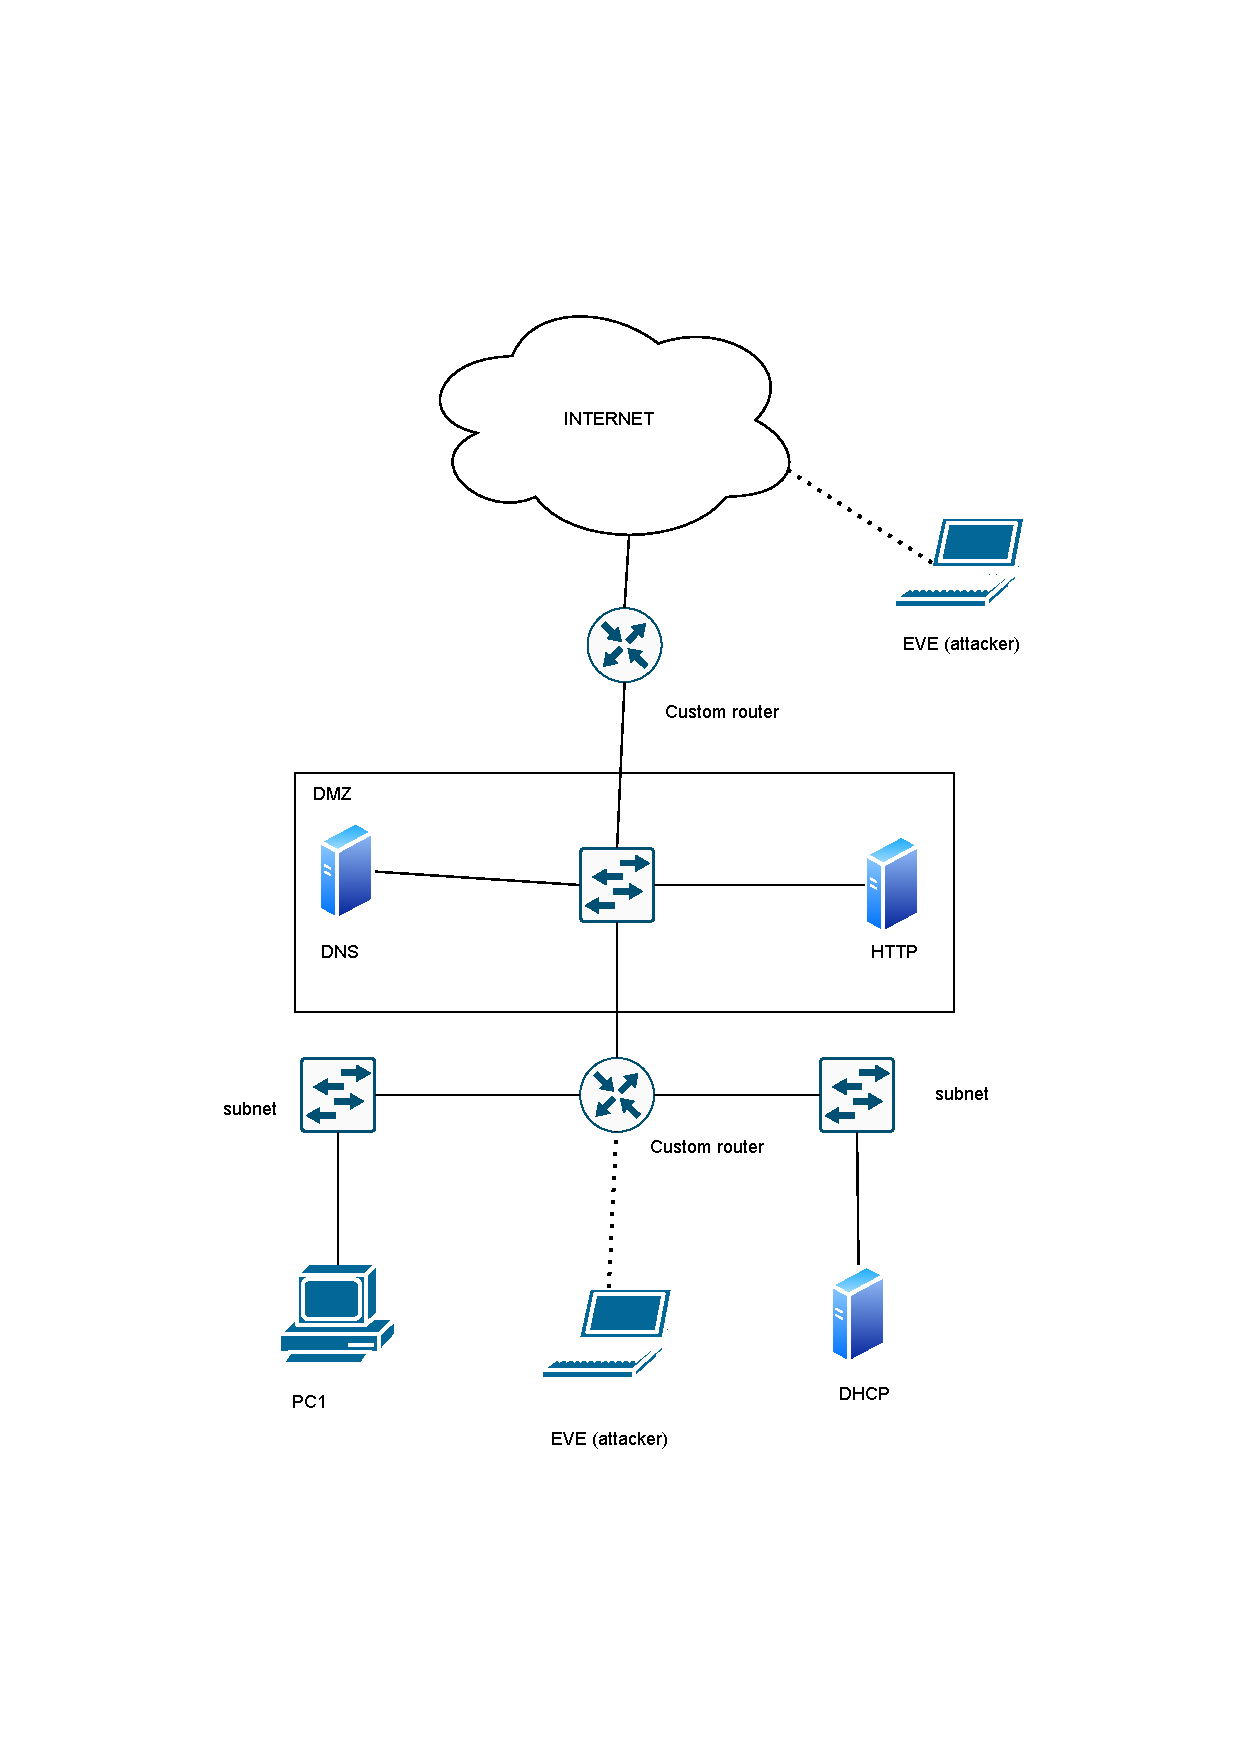
\includegraphics[scale=1.03]{images/architecture_sketch_changed.pdf}
    \caption{Architecture of our project's network}
    \label{fig:1}
\end{figure}
\newpage


\subsection{Appendix 2 : GANTT Diagram}
\label{Appendix2}
\begin{figure}[bp!]
    \centering
    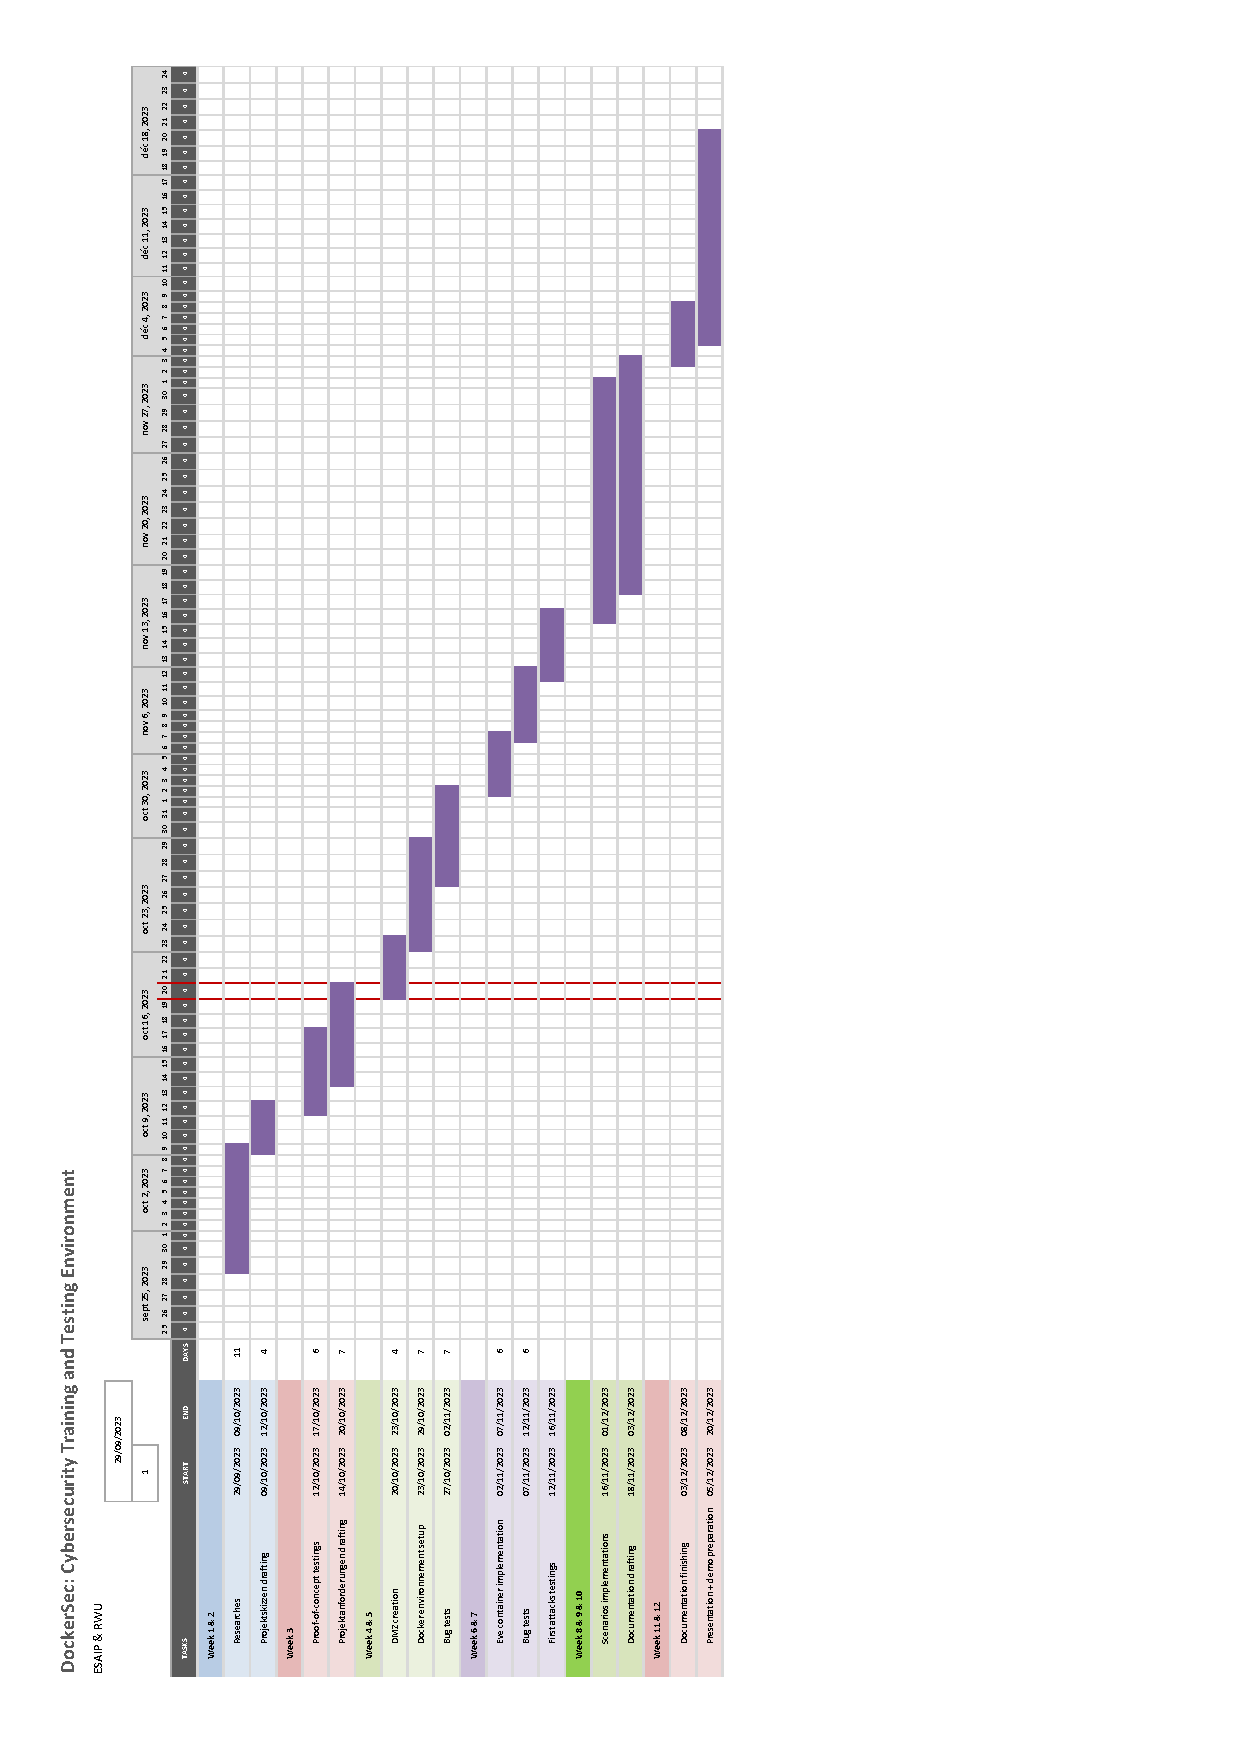
\includegraphics[scale = 0.8]{images/gantt_diagram.pdf}
\end{figure}
\newpage


\end{document}
